\chapter{Symmetrie und Erhaltungssätze}

\lectureoverview{Die stationäre Wirkung und die Euler--Lagrange-Gleichungen bilden eine Hälfte des Herzens der klassischen Mechanik; die Hamiltonsche Formulierung bildet die andere. Hier entwickeln wir die erste Hälfte weit genug, um ein tiefes Muster sichtbar zu machen: Jede kontinuierliche Symmetrie einer Lagrange-Funktion erzeugt eine Erhaltungsgröße. Wir entdecken dieses Muster bei Translationen und Rotationen, beweisen es für eine allgemeine infinitesimale Transformation und untersuchen anschließend sorgfältig, wo das Argument gilt und wo nicht.}

\section{Die minimale Mathematik, die die Physik erklärt}

Die bereits an der Tafel stehenden Zeichen mögen ein wenig an die Schrödinger-Gleichung erinnern, aber darum geht es heute Abend nicht. Das Thema sind Symmetrie und Erhaltung. Ihr Zusammenhang lässt sich nicht auf ehrliche Weise ohne Gleichungen erklären. Die Gleichungen sind elementar; entscheidend ist, sie so anzuordnen, dass die Struktur sichtbar wird. Scientific American mag das Ergebnis benennen, doch hier wollen wir die minimale Mathematik entwickeln, die nötig ist, um es so herzuleiten, wie es Physiker tun würden.

Führen wir einen kleinen Parameter \(\epsilon\) ein. Wir behalten Terme proportional zu \(\epsilon\) bei und verwerfen \(O(\epsilon^2)\). Das ist eine Kurzschreibweise für ein Grenzwertargument und keine Behauptung, das Quadrat einer von null verschiedenen reellen Zahl sei buchstäblich null. Für eine gewöhnliche Funktion \(f(x,y)\) gilt
\begin{equation}
  \delta f
  =\frac{\partial f}{\partial x}\,\delta x
   +\frac{\partial f}{\partial y}\,\delta y
   +O(\epsilon^2),
  \label{eq:first-variation-f}
\end{equation}
wobei sowohl \(\delta x\) als auch \(\delta y\) proportional zu \(\epsilon\) sind. Das Symbol \(\delta f\) bezeichnet die Änderung von \(f\), nicht das Produkt einer Zahl namens \(\delta\) mit \(f\). An einem stationären Punkt gilt
\begin{equation}
  \delta f=0
  \qquad\hbox{to first order.}
  \label{eq:stationary-f}
\end{equation}

Für einen mechanischen Weg \(q_i(t)\) ist die entsprechende Größe die Wirkung
\begin{equation}
  S[q]=\int_{t_1}^{t_2}L(q,\dot q,t)\,dt.
  \label{eq:action-l4}
\end{equation}
Variiert man den Weg bei festgehaltenen Endpunkten, erhält man
\begin{equation}
  \delta S
  =\int_{t_1}^{t_2}dt\,
   \sum_i\left(
     \frac{\partial L}{\partial q_i}\,\delta q_i
     +\frac{\partial L}{\partial\dot q_i}\,\delta\dot q_i
   \right).
  \label{eq:action-variation-l4}
\end{equation}
Die beiden Terme entstehen, weil sich bei einer Änderung des Weges sowohl seine Position als auch seine Geschwindigkeit ändern. Partielle Integration ergibt zusammen mit
\(\delta q_i(t_1)=\delta q_i(t_2)=0\), dass sich \(\delta S=0\) umformen lässt zu
\begin{equation}
  \frac{d}{dt}\left(\frac{\partial L}{\partial\dot q_i}\right)
  -\frac{\partial L}{\partial q_i}=0.
  \label{eq:el-l4}
\end{equation}

\begin{figure}[htbp]
  \centering
  \includegraphics[width=0.76\textwidth]{lecture_04_figure_05.png}
  \caption{Die Euler--Lagrange-Gleichung, hier als Ausgangspunkt für Symmetrie und Erhaltung in Erinnerung gerufen.}
  \lectureframe{00:09:00}
\end{figure}

Die korrekte Bezeichnung lautet \emph{stationäre Wirkung}, nicht unbedingt kleinste Wirkung. Auf diesen Unterschied kommen wir gegen Ende zurück.

\section{Generalisierte Koordinaten und konjugierter Impuls}

Kartesische Positionen sind eine zu enge Sprache für die allgemeine Mechanik. Die Koordinaten können Teilchenpositionen, Winkel, kollektive Variablen oder Feldamplituden sein; deshalb nennen wir sie \(q_i\). Eine Lagrange-Funktion ist eine komprimierte Beschreibung der Dynamik. Selbst das Standardmodell umfasst, ausgeschrieben ohne stark verdichtete Notation, ungefähr eine Seite; für jede Feldkomponente eine eigene Bewegungsgleichung hinzuschreiben, würde erheblich mehr Platz beanspruchen. Die eine Funktion \(L\) fasst sie alle zusammen.

Der zu \(q_i\) konjugierte Impuls ist
\begin{equation}
  p_i=\frac{\partial L}{\partial\dot q_i}.
  \label{eq:canonical-momentum-l4}
\end{equation}
Deshalb nennt man generalisierte Koordinaten traditionell \(q\)-Größen: Die entsprechenden Impulse sind \(p\)-Größen. So erhalten wir unsere \(p\)- und \(q\)-Größen. In dieser Notation wird Gl.~\eqref{eq:el-l4} zu
\begin{equation}
  \dot p_i=\frac{\partial L}{\partial q_i}.
  \label{eq:momentum-el-l4}
\end{equation}

Für das vertraute eindimensionale Teilchen gilt
\begin{equation}
  L=\frac{m\dot x^2}{2}-V(x),
  \qquad
  \frac{\partial L}{\partial\dot x}=m\dot x,
  \label{eq:particle-momentum-l4}
\end{equation}
sodass der konjugierte Impuls der gewöhnliche Impuls ist.

\begin{figure}[htbp]
  \centering
  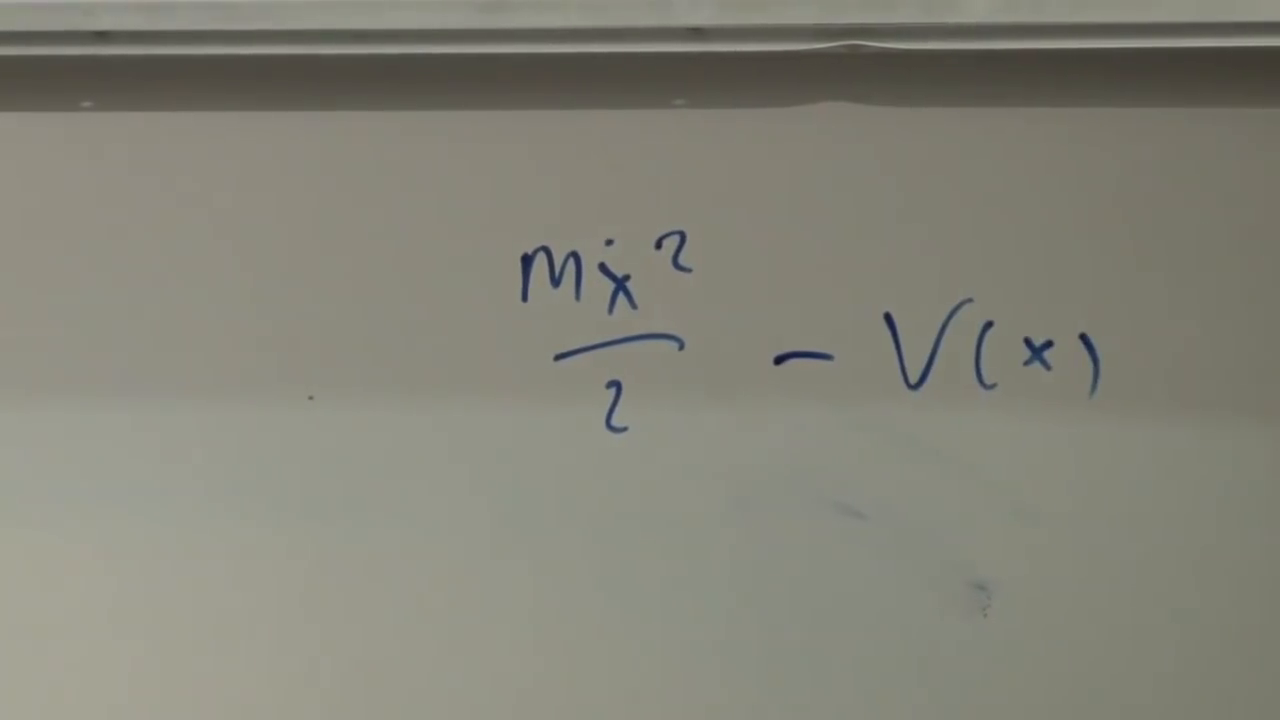
\includegraphics[width=0.72\textwidth]{lecture_04_figure_02.png}
  \caption{Die Lagrange-Funktion als kinetische minus potenzielle Energie, anhand derer der konjugierte Impuls mit \(m\dot x\) identifiziert wird.}
  \lectureframe{00:14:48}
\end{figure}

Wenn \(q_i\) in \(L\) nicht vorkommt, gilt \(\dot p_i=0\). Das ist der vertraute Weg über eine zyklische Koordinate zu einem Erhaltungssatz. Der eigentliche Zusammenhang ist allgemeiner; es ist hilfreich, ihn anhand von Beispielen zu entdecken, bevor wir ihn beweisen.

\section{Erhaltungssätze, bevor wir sie erklären}

\subsection{Zwei Koordinaten und ein nur vom Abstand abhängiges Potenzial}

Setzen wir beide Massen gleich eins und betrachten wir
\begin{equation}
  L=\frac{\dot q_1^{\,2}+\dot q_2^{\,2}}{2}-V(q_1-q_2).
  \label{eq:separation-lagrangian}
\end{equation}
Man kann sich zwei Teilchen auf einer Geraden vorstellen. Ihre Wechselwirkung hängt nur von ihrem Abstand ab.

\begin{figure}[htbp]
  \centering
  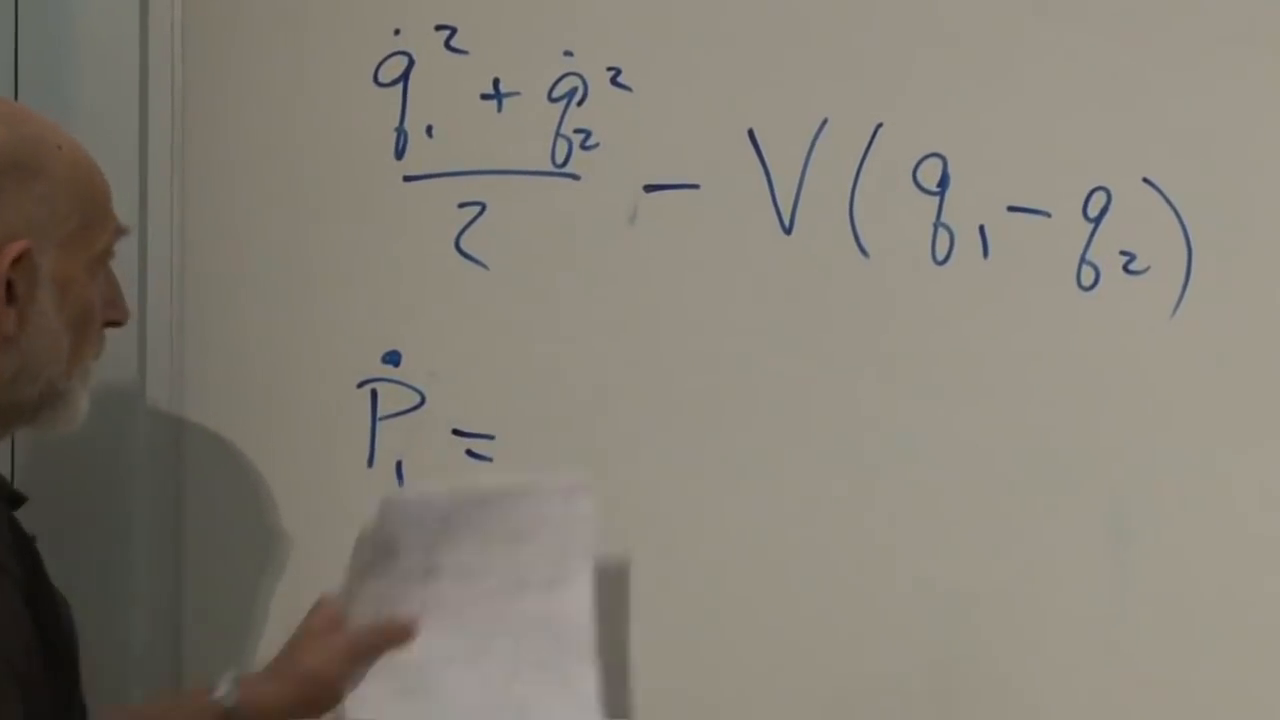
\includegraphics[width=0.78\textwidth]{lecture_04_figure_03.png}
  \caption{Die Lagrange-Funktion für zwei Koordinaten und der Beginn der ersten Impulsgleichung.}
  \lectureframe{00:18:56}
\end{figure}

Schreiben wir \(V'\) für die Ableitung nach dem Argument von \(V\), so gilt
\begin{align}
  \dot p_1&=-V'(q_1-q_2),
  \notag\\
  \dot p_2&=+V'(q_1-q_2).
  \label{eq:separation-momentum-equations}
\end{align}
Das Vorzeichen in der zweiten Gleichung kehrt sich um, weil eine Zunahme von \(q_2\) den Wert von \(q_1-q_2\) verringert.

\begin{classroomqa}
  \audiencequestion{Muss die erste Impulsgleichung \(V'\) enthalten, und woher kommt ihr Minuszeichen?
  \lecturetimestamp{00:20:52--00:21:35}}
  \lecturerresponse{Die Euler--Lagrange-Gleichung besagt
  \(\dot p_1=\partial L/\partial q_1\), nicht, dass die Lagrange-Funktion null ist.
  Da \(L=T-V\) gilt, ergibt die Ableitung nach \(q_1\) den Term
  \(-V'\). Bei der Ableitung nach \(q_2\) kommt durch \(q_1-q_2\) ein weiteres Minuszeichen hinzu, daher steht in der zweiten Gleichung \(+V'\).}
\end{classroomqa}

\begin{figure}[htbp]
  \centering
  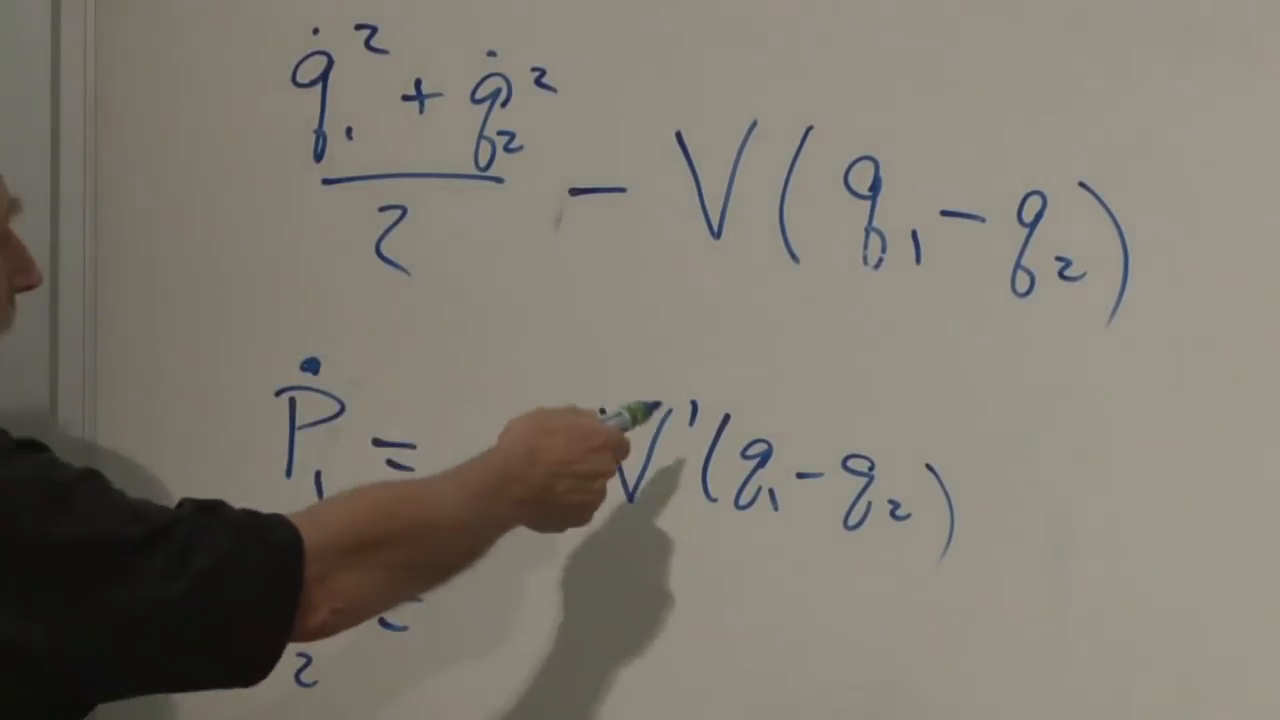
\includegraphics[width=0.78\textwidth]{lecture_04_figure_04.png}
  \caption{Die vorzeichenempfindliche Ableitung in der Gleichung für \(p_1\); in der Gleichung für \(p_2\) ergibt sich das entgegengesetzte Vorzeichen.}
  \lectureframe{00:20:41}
\end{figure}

Addiert man die Gleichungen in ~\eqref{eq:separation-momentum-equations}, erhält man
\begin{equation}
  \frac{d}{dt}(p_1+p_2)=0.
  \label{eq:total-p-conserved}
\end{equation}
Wir haben eine Erhaltungsgröße gefunden, aber noch nicht erklärt, warum sie existiert.

\subsection{Eine weniger offensichtliche Linearkombination}

Betrachten wir nun
\begin{equation}
  L=\frac{\dot q_1^{\,2}+\dot q_2^{\,2}}{2}
    -V(Aq_1+Bq_2),
  \label{eq:ab-lagrangian}
\end{equation}
wobei \(A\) und \(B\) Konstanten sind. Dann gilt
\begin{align}
  \dot p_1&=-A\,V'(Aq_1+Bq_2),
  \notag\\
  \dot p_2&=-B\,V'(Aq_1+Bq_2).
  \label{eq:ab-momentum-equations}
\end{align}
Multipliziert man die erste Gleichung mit \(B\), die zweite mit \(A\) und subtrahiert die Gleichungen, so fällt die Kraft heraus:
\begin{equation}
  \frac{d}{dt}(Bp_1-Ap_2)=0.
  \label{eq:ab-conserved}
\end{equation}

\begin{figure}[htbp]
  \centering
  \includegraphics[width=0.78\textwidth]{lecture_04_figure_06.png}
  \caption{Die gewichteten Impulsgleichungen, deren Kraftterme sich in \(Bp_1-Ap_2\) aufheben.}
  \lectureframe{00:24:20}
\end{figure}

\begin{classroomqa}
  \audiencequestion{Woher könnten Konstanten wie \(A\) und \(B\) physikalisch kommen?\lecturetimestamp{00:25:09--00:30:15}}
  \lecturerresponse{Betrachten wir zwei Teilchen mit den Massen \(m\) und \(M\):
  \[
    L=\frac{m\dot X^2}{2}+\frac{M\dot Y^2}{2}-V(X-Y).
  \]
  Skalieren wir um zu \(Q_1=\sqrt m\,X\) und \(Q_2=\sqrt M\,Y\). Der kinetische Term wird zu \((\dot Q_1^2+\dot Q_2^2)/2\), während das Potenzial von \(Q_1/\sqrt m-Q_2/\sqrt M\) abhängt. Ungleiche Massen treten somit ganz natürlich als Koeffizienten einer Linearkombination auf. Ersetzt man \(Q_2\) durch \(-Q_2\), wird aus dem dargestellten Minus ein Plus, ohne den quadrierten kinetischen Term zu verändern.}
\end{classroomqa}

\begin{figure}[htbp]
  \centering
  \includegraphics[width=0.82\textwidth]{lecture_04_figure_07.png}
  \caption{Massengewichtete Koordinaten vereinfachen die kinetische Energie und verlagern die Massenfaktoren ins Potenzial.}
  \lectureframe{00:28:40}
\end{figure}

\begin{classroomqa}
  \audiencequestion{Zeigt dies, dass eine Erhaltungsgröße auch ohne zyklische Koordinate existieren kann?\lecturetimestamp{00:31:13--00:31:58}}
  \lecturerresponse{In den hier verwendeten Variablen gibt es keine \emph{offensichtliche} zyklische Koordinate. Eine Variablentransformation könnte eine solche sichtbar machen, doch danach zu suchen, ist hier nicht der hilfreiche Blickwinkel. Das Symmetrieargument wird die erhaltene Kombination direkt identifizieren.}
\end{classroomqa}

\section{Was wir unter einer Symmetrie verstehen}

\subsection{Translationen}

Beginnen wir mit einem freien Teilchen der Masse eins,
\begin{equation}
  L=\frac{\dot q^2}{2}.
  \label{eq:free-unit-l4}
\end{equation}
und verschieben wir jeden Punkt seiner Bahn um dieselbe Konstante:
\begin{equation}
  q'(t)=q(t)+\epsilon.
  \label{eq:free-translation}
\end{equation}
Da \(\epsilon\) zeitunabhängig ist, gilt \(\dot q'=\dot q\) und somit
\(\delta L=0\). Diese Invarianz ist Translationssymmetrie.

Es gibt zwei gleichwertige Sichtweisen. Bei der passiven Beschreibung verschiebt man den Koordinatenursprung, während das Objekt an seinem Platz bleibt. Bei der aktiven Beschreibung bleiben die Achsen fest und das Objekt wird bewegt. Die aktive Ausdrucksweise ist weniger verwirrend: Wir verändern die physikalische Konfiguration und fragen, ob \(L\) davon etwas bemerkt.

Für Gl.~\eqref{eq:separation-lagrangian} verschieben wir beide Koordinaten:
\begin{equation}
  \delta q_1=\epsilon,
  \qquad
  \delta q_2=\epsilon.
  \label{eq:common-translation}
\end{equation}
Die Geschwindigkeiten bleiben unverändert, ebenso \(q_1-q_2\).

\begin{figure}[htbp]
  \centering
  \includegraphics[width=0.78\textwidth]{lecture_04_figure_08.png}
  \caption{Eine gemeinsame Translation lässt den Abstand zwischen zwei Koordinaten unverändert.}
  \lectureframe{00:35:30}
\end{figure}

Für Gl.~\eqref{eq:ab-lagrangian} verwenden wir die weniger offensichtliche Transformation
\begin{equation}
  \delta q_1=B\epsilon,
  \qquad
  \delta q_2=-A\epsilon.
  \label{eq:ab-transformation}
\end{equation}
Auch hier ändern sich die Geschwindigkeiten nicht, während
\begin{equation}
  \delta(Aq_1+Bq_2)=AB\epsilon-BA\epsilon=0.
  \label{eq:ab-invariant-argument}
\end{equation}
Damit ist diese Transformation eine Symmetrie.

\begin{figure}[htbp]
  \centering
  \includegraphics[width=0.80\textwidth]{lecture_04_figure_09.png}
  \caption{Die asymmetrische Translation, die \(Aq_1+Bq_2\) erhält.}
  \lectureframe{00:40:20}
\end{figure}

\begin{classroomqa}
  \audiencequestion{Codieren die Koeffizienten die Massen, sodass die Erhaltungsgröße zum gewöhnlichen Schwerpunktsimpuls wird?\lecturetimestamp{00:42:25--00:42:45}}
  \lecturerresponse{Ja. In den massengewichteten Variablen erscheinen die Symmetrie und die erhaltene Kombination asymmetrisch. Transformiert man zurück zu \(X\) und \(Y\), erhält man wieder die gewöhnliche gleichzeitige Translation und den Gesamtimpuls.}
\end{classroomqa}

\subsection{Rotationen}

Betrachten wir ein Teilchen in der Ebene,
\begin{equation}
  L=\frac{m}{2}(\dot x^2+\dot y^2)-V(x^2+y^2).
  \label{eq:central-lagrangian-l4}
\end{equation}
Dies ist ein Zentralpotenzial. Wir vergleichen zwei feste Koordinatensysteme, die gegeneinander gedreht sind; die Achsen rotieren nicht mit der Zeit. Bei einer konsistenten Wahl der Orientierung gilt
\begin{align}
  x'&=x\cos\theta+y\sin\theta,
  \notag\\
  y'&=-x\sin\theta+y\cos\theta.
  \label{eq:finite-rotation-l4}
\end{align}

\begin{figure}[htbp]
  \centering
  \includegraphics[width=0.82\textwidth]{lecture_04_figure_10.png}
  \caption{Eine Lagrange-Funktion für ein Zentralpotenzial und zwei feste kartesische Bezugssysteme, die durch eine Rotation miteinander verbunden sind.}
  \lectureframe{00:45:40}
\end{figure}

Setzen wir \(\theta=\epsilon\) und behalten wir nur Terme erster Ordnung:
\begin{equation}
  \cos\epsilon=1+O(\epsilon^2),
  \qquad
  \sin\epsilon=\epsilon+O(\epsilon^3).
  \label{eq:small-angle-l4}
\end{equation}
Die infinitesimale Rotation lautet
\begin{align}
  \delta x&=y\epsilon,
  &\delta y&=-x\epsilon,
  \notag\\
  \delta\dot x&=\dot y\epsilon,
  &\delta\dot y&=-\dot x\epsilon.
  \label{eq:infinitesimal-rotation-l4}
\end{align}

\begin{figure}[htbp]
  \centering
  \includegraphics[width=0.82\textwidth]{lecture_04_figure_11.png}
  \caption{Die infinitesimale Rotation der Koordinaten und Geschwindigkeiten.}
  \lectureframe{00:49:50}
\end{figure}

Anders als bei einer Translation hängt die Änderung von \(x\) von \(y\) ab; die Änderung von \(y\) wiederum hängt von \(x\) ab. Dennoch gilt
\begin{align}
  \delta(x^2+y^2)
  &=2x\,\delta x+2y\,\delta y=0,
  \notag\\
  \delta(\dot x^2+\dot y^2)
  &=2\dot x\,\delta\dot x+2\dot y\,\delta\dot y=0.
  \label{eq:rotation-invariants-l4}
\end{align}
Sowohl der Potenzialterm als auch der kinetische Term sind invariant.

\begin{figure}[htbp]
  \centering
  \includegraphics[width=0.76\textwidth]{lecture_04_figure_12.png}
  \caption{Die Aufhebung der Terme erster Ordnung zeigt, dass das Quadrat des Radius rotationsinvariant ist.}
  \lectureframe{00:53:20}
\end{figure}

\section{Der allgemeine Erhaltungssatz}

Die Beispiele der Translation und Rotation lassen sich auf dieselbe Weise darstellen. Sei eine kontinuierliche infinitesimale Transformation gegeben durch
\begin{equation}
  \delta q_i=\epsilon f_i(q),
  \qquad
  \delta\dot q_i=\frac{d}{dt}\delta q_i,
  \label{eq:general-infinitesimal-symmetry}
\end{equation}
wobei \(\epsilon\) zeitunabhängig ist und \(f_i\) von allen Koordinaten abhängen kann.

\begin{figure}[htbp]
  \centering
  \includegraphics[width=0.78\textwidth]{lecture_04_figure_13.png}
  \caption{Ein allgemeines infinitesimales Verschiebungsfeld \(\delta q_i=\epsilon f_i(q)\).}
  \lectureframe{00:56:00}
\end{figure}

Die Variation der Lagrange-Funktion erster Ordnung ist
\begin{equation}
  \delta L
  =\sum_i\left(
    \frac{\partial L}{\partial q_i}\delta q_i
    +\frac{\partial L}{\partial\dot q_i}\delta\dot q_i
  \right).
  \label{eq:delta-l-general}
\end{equation}

\begin{figure}[htbp]
  \centering
  \includegraphics[width=0.84\textwidth]{lecture_04_figure_14.png}
  \caption{Die beiden Beiträge zu \(\delta L\): Variation der Koordinaten und Variation der Geschwindigkeiten.}
  \lectureframe{01:02:30}
\end{figure}

Betrachten wir nun eine physikalische Bahn, auf der die Euler--Lagrange-Gleichungen gelten. Mit
\begin{equation}
  \frac{\partial L}{\partial\dot q_i}=p_i,
  \qquad
  \frac{\partial L}{\partial q_i}=\dot p_i,
  \label{eq:el-substitution-l4}
\end{equation}
erhalten wir
\begin{align}
  \delta L
  &=\sum_i\left(\dot p_i\,\delta q_i
                +p_i\,\delta\dot q_i\right)
  \notag\\
  &=\frac{d}{dt}\sum_i p_i\delta q_i
  =\epsilon\frac{d}{dt}\sum_i p_i f_i(q).
  \label{eq:noether-derivation-l4}
\end{align}
Der zentrale Schritt besteht lediglich in der Produktregel.

Ist die Transformation eine Symmetrie, gilt \(\delta L=0\). Da \(\epsilon\) ein beliebiger konstanter Faktor ist, folgt
\begin{equation}
  \boxed{
  \frac{d\mathcal Q}{dt}=0,
  \qquad
  \mathcal Q=\sum_i p_i f_i(q)}
  .
  \label{eq:noether-charge-l4}
\end{equation}
Dies ist der kernmechanische Teil des Satzes von Noether für exakte, zeitunabhängige Punktsymmetrien.

\begin{figure}[htbp]
  \centering
  \includegraphics[width=0.84\textwidth]{lecture_04_figure_15.png}
  \caption{Der Schritt mit der Produktregel, der die Invarianz von \(L\) in eine Erhaltungsgröße überführt.}
  \lectureframe{01:05:00}
\end{figure}

\begin{classroomqa}
  \audiencequestion{Trägt \(q\) in \(f_i(q)\) noch einen weiteren Index?
  \lecturetimestamp{01:06:57--01:07:31}}
  \lecturerresponse{Das nicht indizierte \(q\) bezeichnet die gesamte Menge
  \((q_1,q_2,\ldots)\). Jede Komponente \(f_i\) kann von all diesen
  Koordinaten abhängen. Bei einer Rotation gilt zum Beispiel \(f_x=y\) und \(f_y=-x\).}
\end{classroomqa}

Die Beispiele sind nun keine Zufälle mehr. Für eine gemeinsame Translation gilt \(f_1=f_2=1\), also
\begin{equation}
  \mathcal Q=p_1+p_2.
  \label{eq:noether-common-p}
\end{equation}
Für die asymmetrische Translation gilt \(f_1=B\), \(f_2=-A\), also
\begin{equation}
  \mathcal Q=Bp_1-Ap_2.
  \label{eq:noether-ab-p}
\end{equation}
Bei einer Rotation gilt \(f_x=y\) und \(f_y=-x\):
\begin{equation}
  \mathcal Q=p_xy-p_yx.
  \label{eq:rotation-charge-sign}
\end{equation}
Bis auf das Vorzeichen, das von der Orientierung abhängt, ist dies der Drehimpuls,
\begin{equation}
  J=xp_y-yp_x.
  \label{eq:angular-momentum-l4}
\end{equation}

\begin{figure}[htbp]
  \centering
  \includegraphics[width=0.82\textwidth]{lecture_04_figure_16.png}
  \caption{Die Noether-Ladung der Rotation, die bis auf die Orientierung dem Drehimpuls in der Ebene entspricht.}
  \lectureframe{01:11:00}
\end{figure}

Bei vielen wechselwirkenden Teilchen drehen wir alle Teilchen gemeinsam. Aufgrund der Invarianz bleibt dann die Summe ihrer Drehimpulse erhalten, nicht aber der Drehimpuls jedes einzelnen Teilchens für sich.

\section{Fragen zu den Voraussetzungen des Satzes}

\begin{classroomqa}
  \audiencequestion{Führt ein rotierendes Koordinatensystem zu einer expliziten Zeitabhängigkeit von \(\delta L\)?\lecturetimestamp{01:12:57--01:13:57}}
  \lecturerresponse{Ja. Der eben geführte Beweis setzt einen zeitunabhängigen Symmetrieparameter voraus: eine feste Translation oder eine feste Rotation. Bei einer Transformation mit zeitabhängigem Parameter treten zusätzliche Terme auf; dann ist eine allgemeinere Behandlung nötig.}
\end{classroomqa}

\begin{classroomqa}
  \audiencequestion{Bezeichnet das große \(Q\) in der Formel an der Tafel die Transformation selbst?\lecturetimestamp{01:14:02--01:15:58}}
  \lecturerresponse{Nein. Diese Notation kollidiert leider mit den Koordinaten \(q_i\). Die Transformation ist \(\delta q_i=\epsilon f_i(q)\); die daraus hervorgehende Erhaltungsgröße ist \(\mathcal Q=\sum_i p_i f_i\). Der Koeffizient \(f_i\) gibt an, wie sich die \(i\)-te Koordinate unter der Symmetrie verändert.}
\end{classroomqa}

Auch die Energieerhaltung wird durch eine Symmetrie erzeugt, aber durch eine andere: die Translation in der Zeit, also die Unabhängigkeit davon, wo der Zeitnullpunkt liegt. Dieser Fall und die Hamiltonsche Formulierung werden später behandelt.

\begin{classroomqa}
  \audiencequestion{Könnte man die tatsächliche Bewegung in ein veränderliches Koordinatensystem aufnehmen, sodass die Mechanik nur noch aus Koordinatentransformationen besteht?\lecturetimestamp{01:17:43--01:20:01}}
  \lecturerresponse{Man kann Koordinaten wählen, die einer bestimmten Bewegung folgen. Dann hängt die Transformation aber vom Anfangszustand und von der Bahn ab. Die hier verwendete Symmetrietransformation ist unabhängig davon festgelegt, welcher Lösung das System folgt. Die Bewegung selbst lässt sich natürlicher im gemeinsamen Raum der Koordinaten und Impulse darstellen.}
\end{classroomqa}

\section{Der harmonische Oszillator im Phasenraum}

Bei Masse und Federkonstante gleich eins gilt
\begin{equation}
  L=\frac{\dot q^2}{2}-\frac{q^2}{2}.
  \label{eq:oscillator-l4}
\end{equation}
Der konjugierte Impuls und die Bewegungsgleichung lauten
\begin{equation}
  p=\dot q,
  \qquad
  \dot p=-q,
  \label{eq:oscillator-first-order-l4}
\end{equation}
oder
\begin{equation}
  \dot q=p,
  \qquad
  \dot p=-q.
  \label{eq:oscillator-phase-flow}
\end{equation}
Diese Gleichungen beschreiben eine gleichförmige Kreisbewegung in der \(q\)-\(p\)-Ebene. Die Hin-und-her-Bewegung des Oszillators im Ortsraum ist die Projektion dieses Kreises auf die \(q\)-Achse: Bei \(q=0\) ist die Geschwindigkeit am größten und an den Umkehrpunkten null.

\begin{figure}[htbp]
  \centering
  \includegraphics[width=0.82\textwidth]{lecture_04_figure_17.png}
  \caption{Die Gleichungen des harmonischen Oszillators und seine Kreisbahn im \(q\)-\(p\)-Raum.}
  \lectureframe{01:25:30}
\end{figure}

\begin{classroomqa}
  \audiencequestion{Läuft die Kreisbahn im Phasenraum im Uhrzeigersinn?\lecturetimestamp{01:25:47--01:27:15}}
  \lecturerresponse{Wenn \(p\) horizontal und \(q\) vertikal aufgetragen wird, ja. Bei maximal positivem \(q\) gilt \(\dot p=-q<0\), die Bewegung weist also nach unten. Vertauscht man die Anordnung der Achsen, kehrt sich der visuelle Drehsinn um. Deshalb kann man sich die Konvention leicht falsch merken.}
\end{classroomqa}

Das Paar in Gl.~\eqref{eq:oscillator-phase-flow} ähnelt bereits den Hamilton-Gleichungen, wurde aber vollständig im Rahmen der Lagrange-Mechanik hergeleitet.

\section{Kontinuierliche und diskrete Symmetrien}

\begin{classroomqa}
  \audiencequestion{Muss eine Symmetrie durch eine infinitesimale kartesische Transformation ausgedrückt werden?\lecturetimestamp{01:27:48--01:30:31}}
  \lecturerresponse{Kartesische Koordinaten sind lediglich praktisch; für diesen Beweis ist Kontinuität die wesentliche Voraussetzung. Manche Symmetrien haben keine infinitesimale Version. Bei einem geraden Potenzial werden \(q\mapsto -q\) und \(\dot q\mapsto-\dot q\) abgebildet, wobei \(L\) unverändert bleibt. Eine Spiegelung lässt sich jedoch nicht aus beliebig kleinen Spiegelungen zusammensetzen. Diese klassische Herleitung liefert daher keine zugehörige Erhaltungsgröße.}
\end{classroomqa}

\begin{figure}[htbp]
  \centering
  \includegraphics[width=0.82\textwidth]{lecture_04_figure_18.png}
  \caption{Ein gerades Potenzial ist unter der diskreten Spiegelung \(q\mapsto -q\) invariant.}
  \lectureframe{01:29:30}
\end{figure}

\begin{classroomqa}
  \audiencequestion{Zeigt eine von null verschiedene Erhaltungsgröße \(\mathcal Q\), dass die Transformation keine Symmetrie war?\lecturetimestamp{01:30:40--01:31:30}}
  \lecturerresponse{Nein. Eine Erhaltungsgröße kann jeden beliebigen konstanten Wert haben. Entscheidend ist die Prüfung, ob \(\dot{\mathcal Q}\) gilt. Ist die aus einer vorgeschlagenen Transformation hergeleitete Größe nicht erhalten, so war diese Transformation unter den Voraussetzungen des Beweises keine Symmetrie.}
\end{classroomqa}

\begin{classroomqa}
  \audiencequestion{Die Spiegelung lässt die Lagrange-Funktion weiterhin unverändert. Warum ergibt sich daraus also kein Erhaltungssatz?\lecturetimestamp{01:31:34--01:32:27}}
  \lecturerresponse{Die Invarianz ist zwar erkennbar, doch die Herleitung führte über eine Verschiebung erster Ordnung und die Produktregel. Eine Spiegelung bringt einen mit einem einzigen diskreten Schritt von der einen Seite des Konfigurationsraums auf die andere. Ohne einen infinitesimalen Generator \(f_i\) hat die Formel \(\mathcal Q=\sum_i p_i f_i\) nichts, worauf sie angewendet werden könnte.}
\end{classroomqa}

\begin{classroomqa}
  \audiencequestion{Wie heißt die Eigenschaft, aus beliebig kleinen Transformationen aufgebaut zu sein?\lecturetimestamp{01:32:36--01:33:23}}
  \lecturerresponse{Das ist eine \emph{kontinuierliche Symmetrie}. Translation und Rotation sind kontinuierlich; die Spiegelung ist eine \emph{diskrete Symmetrie}.}
\end{classroomqa}

\begin{classroomqa}
  \audiencequestion{Können sich verworfene Fehler der Ordnung \(O(\epsilon^2)\) aufsummieren, wenn viele infinitesimale Schritte eine endliche Transformation ergeben?\lecturetimestamp{01:33:23--01:36:10}}
  \lecturerresponse{Die infinitesimale Invarianz muss an jedem Punkt gelten, der entlang der Transformation erreicht wird, nicht nur am Ausgangspunkt. Teilen wir ein endliches Parameterintervall in \(N\) Schritte der Größe \(\epsilon\) auf: Die aufsummierte Verschiebung erster Ordnung beträgt \(N\epsilon\), während sich ein lokaler Restterm der Ordnung \(O(\epsilon^2)\) zu \(N\epsilon^2=(N\epsilon)\epsilon\to0\) aufsummiert. Diese Übertragung vom Lokalen aufs Endliche wird durch kontinuierliche Transformationsgruppen formalisiert.}
\end{classroomqa}

\begin{classroomqa}
  \audiencequestion{Kommen diskrete Symmetrien in klassischen Systemen tatsächlich vor?\lecturetimestamp{01:36:32--01:37:25}}
  \lecturerresponse{Gewiss. Der harmonische Oszillator selbst besitzt das gerade Potenzial \(V(q)\propto q^2\) und ist daher unter \(q\mapsto -q\) invariant. Es gibt viele solche Beispiele; entscheidend ist nur, dass diese diskrete Invarianz keine neue klassische Noether-Ladung liefert.}
\end{classroomqa}

\begin{classroomqa}
  \audiencequestion{Wenn sowohl kontinuierliche als auch diskrete Transformationen \(L\) unverändert lassen, ist das dann nicht dieselbe Bedingung?\lecturetimestamp{01:37:37--01:39:18}}
  \lecturerresponse{Als endliche Aussage über Invarianz ist es dieselbe Bedingung, aber nicht derselbe mathematische Ausgangspunkt für diesen Beweis. Der Beweis benötigt eine Variation erster Ordnung. Bei einer Spiegelung hat der Ausdruck erste Ordnung keine Bedeutung; die Gleichungskette, die zu einer Ladung führt, lässt sich daher gar nicht erst beginnen.}
\end{classroomqa}

\begin{classroomqa}
  \audiencequestion{Wie hängt dies historisch mit dem Satz von Noether zusammen?\lecturetimestamp{01:39:26--01:40:42}}
  \lecturerresponse{Dies ist ein eingeschränkter Teil von Emmy Noethers wesentlich allgemeinerem Satz. Einzelne Zusammenhänge zwischen Symmetrien und Erhaltungsgrößen waren bereits früher bekannt, doch Noether fasste sie Anfang des zwanzigsten Jahrhunderts in einem einheitlichen und bemerkenswert allgemeinen Rahmen zusammen. Ihrer mathematischen Bedeutung wurde akademisch nicht in angemessener Weise Rechnung getragen.}
\end{classroomqa}

\begin{classroomqa}
  \audiencequestion{Ist die klassische Mechanik noch ein aktives Forschungsgebiet?\lecturetimestamp{01:40:47--01:42:37}}
  \lecturerresponse{Ja. Der hier verwendete elementare Satz ist alt, doch nichtlineare Dynamik, integrierbare Systeme, Chaos, Strömungsmechanik und geometrische Mechanik sind weiterhin lebendige Forschungsgebiete. Das Symmetrieprinzip reicht zudem weit über die klassische Teilchenmechanik hinaus.}
\end{classroomqa}

\section{Warum das Wirkungsprinzip wichtig ist}

\begin{classroomqa}
  \audiencequestion{Gibt es einen anschaulichen Grund dafür, dass Symmetrie Erhaltung zur Folge haben sollte?\lecturetimestamp{01:42:49--01:47:57}}
  \lecturerresponse{Nicht allein aufgrund der Symmetrie. Betrachten wir den viskosen Widerstand,
\[
    m\ddot x=-c\dot x.
  \]
Die Gleichung ist unter \(x\mapsto x+\epsilon\) invariant. Für \(p=m\dot x\) gilt jedoch
\[
    \dot p=-\frac{c}{m}p,
    \qquad
    p(t)=p(0)e^{-ct/m},
  \]
sodass der Impuls abnimmt. Dies ist eine effektive Gleichung für ein Teilsystem und kein fundamentales Prinzip stationärer Wirkung für \(x\) allein. Bezieht man die Flüssigkeitsmoleküle und den Rest des abgeschlossenen Systems ein, bleibt der Gesamtimpuls erhalten. Symmetrie und Erhaltung hängen über das Wirkungsprinzip der Lagrange-Mechanik zusammen, nicht allein über die Gestalt einer Differentialgleichung.}
\end{classroomqa}

\begin{figure}[htbp]
  \centering
  \includegraphics[width=0.65\textwidth]{lecture_04_figure_19.png}
  \caption{Translationsinvarianter viskoser Widerstand, bei dem der Impuls des reduzierten Teilchens dennoch abnimmt.}
  \lectureframe{01:44:30}
\end{figure}

\begin{classroomqa}
  \audiencequestion{Lässt sich quantifizieren, wann die physikalische Bahn kein Minimum der Wirkung ist?\lecturetimestamp{01:48:08--01:51:38}}
  \lecturerresponse{Ein echtes Minimum ist die Ausnahme; im Allgemeinen ist die Wirkung im Raum der Wege ein Sattel. Für den Oszillator mit Masse und Federkonstante eins gilt
  \[
    S[q]=\frac12\int(\dot q^2-q^2)\,dt.
  \]
Eine schmale, sich rasch ändernde Deformation erhöht den positiven Beitrag \(\dot q^2\). Eine breite Deformation, bei der der Weg lange Zeit leicht ausgelenkt bleibt, kann den negativen Beitrag \(-q^2\) überwiegen lassen und die Wirkung verringern. Dieselbe stationäre Bahn hat somit Richtungen, in denen die Wirkung zunimmt, und andere, in denen sie abnimmt. Die Quantenmechanik liefert durch die Sichtweise des Pfadintegrals den tieferen Ursprung der Stationarität; dieses Argument behandeln wir jedoch später.}
\end{classroomqa}

\begin{figure}[htbp]
  \centering
  \includegraphics[width=0.80\textwidth]{lecture_04_figure_20.png}
  \caption{Ein benachbarter, breit ausgelenkter Weg des Oszillators veranschaulicht, warum die stationäre Wirkung typischerweise ein Sattel und kein Minimum ist.}
  \lectureframe{01:50:20}
\end{figure}

\begin{classroomqa}
  \audiencequestion{Gibt es eine eineindeutige Zuordnung zwischen kontinuierlichen Symmetrien und Erhaltungssätzen?\lecturetimestamp{01:51:44--01:52:43}}
  \lecturerresponse{Im Rahmen der Variationsrechnung und nach Identifizierung äquivalenter oder trivialer Fälle trifft dieses Bild im Wesentlichen zu. Zu jeder kontinuierlichen Symmetrie gehört eine Ladung, und Erhaltungsgrößen lassen sich im Allgemeinen auf Symmetrien zurückführen. Präzise Formulierungen bringen technische Einschränkungen mit sich; die allgemeine Aussage sollte daher nicht unbedacht verwendet werden.}
\end{classroomqa}

\begin{classroomqa}
  \audiencequestion{Muss jede Lagrange-Funktion eine nichttriviale Symmetrie besitzen?\lecturetimestamp{01:52:43--01:53:23}}
  \lecturerresponse{Nein. Die Beispiele wurden so gewählt, dass sie Symmetrien besitzen. Eine generische Lagrange-Funktion muss unter keiner der vorgeschlagenen räumlichen Transformationen invariant sein.}
\end{classroomqa}

\begin{classroomqa}
  \audiencequestion{Sollte man eine Symmetrie letztlich als aktive Bewegung oder als passive Koordinatenänderung verstehen?\lecturetimestamp{01:53:25--01:55:08}}
  \lecturerresponse{Beide Beschreibungen lassen sich gleichwertig formulieren, doch die aktive ist hier klarer. Wir bewegen das gesamte physikalische System und fragen, ob sich die Lagrange-Funktion ändert. In der passiven Ausdrucksweise muss man stattdessen sagen, dass die \emph{Form} der Lagrange-Funktion unverändert bleibt, wenn sich das Koordinatensystem bewegt.}
\end{classroomqa}

\begin{classroomqa}
  \audiencequestion{Was kommt als Nächstes?\lecturetimestamp{01:55:10--01:55:35}}
  \lecturerresponse{Die Energieerhaltung, ihr Ursprung in der Zeittranslationssymmetrie und anschließend die Hamiltonsche Formulierung.}
\end{classroomqa}
